\documentclass{homework}

\input{particulars}

\sisetup{round-precision=3}

\renewcommand\thesubsection{\arabic{subsection}}
\renewcommand\thesubsubsection{\thesubsection.\arabic{subsubsection}}

\begin{document}

\title{Machine Learning Homework \#5}
\author{\chineseName \masterStudentID}
\date{}
\maketitle

\section{Gaussian Process}

\subsection{Code}

\subsubsection{Task 1}

The imported modules are:

\begin{lstlisting}[language=Python]
import numpy as np
import matplotlib.pyplot as plt
from scipy.optimize import minimize
from scipy.spatial.distance import cdist
\end{lstlisting}

% The rational quadratic kernel is a generalization of the squared exponential kernel, which can model varying length-scales across different parts of the input space.

The rational quadratic kernel is defined as:

\[
k(x, x') = \left(1 + \frac{\|x - x'\|^2}{2\alpha l^2}\right)^{-\alpha}
\]

Where:

\begin{itemize}
    \item \( \|x - x'\|^2 \): squared Euclidean distance between the input points.
    \item \( l \): length scale parameter that controls the smoothness of the kernel.
    \item \( \alpha \): a parameter that controls the relative importance of the squared distances.
\end{itemize}

\begin{lstlisting}[language=Python]
def rational_quadratic_kernel(X1, X2, length_scale=1.0, alpha=1.0):
    # squared Euclidean distances between each pair of points in X1 and X2
    dists = cdist(X1, X2, metric='sqeuclidean')
    # rational quadratic kernel matrix
    return (1 + dists / (2 * alpha * length_scale**2))**(-alpha)
\end{lstlisting}

% This function implements the Gaussian Process model, which predicts the mean and covariance of the function value at test points, based on training data.
This function implements the Gaussian Process model.

The GP regression model is:

\[
\mu_* = K_*(K + \sigma_n^2 I)^{-1} y
\]
\[
\Sigma_* = K_{**} - K_*^T(K + \sigma_n^2 I)^{-1}K_*
\]

Where:

\begin{itemize}
    \item \( \mu_* \): mean prediction at test points.
    \item \( \Sigma_* \): covariance of the prediction.
    \item \( K \): kernel matrix computed on the training points.
    \item \( K_* \): cross-covariance matrix between the training and prediction points.
    \item \( K_{**} \): kernel matrix between the prediction points.
    \item \( y \): vector of observed training values.
    \item \( \sigma_n^2 \): noise variance.
\end{itemize}

\begin{lstlisting}[language=Python]
def gaussian_process(X_train, Y_train, X_pred, kernel, beta=5, params=None):
    if params is None:
        # default kernel parameters
        params = {'length_scale': 1.0, 'alpha': 1.0}
    
    # kernel matrix K
    K = kernel(X_train, X_train, **params) + np.eye(len(X_train)) / beta
    # cross-covariance matrix K_*
    K_s = kernel(X_train, X_pred, **params)
    # kernel matrix K_**
    K_ss = kernel(X_pred, X_pred, **params) + np.eye(len(X_pred)) * 1e-8
    
    # caculate posterior mean and covariance
    K_inv = np.linalg.inv(K)
    mu = K_s.T @ K_inv @ Y_train
    cov = K_ss - K_s.T @ K_inv @ K_s
    
    return mu, cov
\end{lstlisting}

% The Negative Log Marginal Likelihood (NLL) is used as an objective function to optimize the kernel parameters in the Gaussian Process.
This function implements Negative Log Marginal Likelihood (NLL).

% Minimizing this function corresponds to finding the parameters that best explain the observed data.

The NLL function for GP is given by:

\[
\text{NLL} = \frac{1}{2} y^T K^{-1} y + \frac{1}{2} \log |K| + \frac{n}{2} \log 2 \pi
\]

Where:

\begin{itemize}
    \item \( K \): kernel matrix% with added noise term.
    \item \( y \): vector of observed outputs.
    \item \( n \): number of training points.
\end{itemize}

\subsubsection{Task 2}

\begin{lstlisting}[language=Python]
# Negative Log Marginal Likelihood (NLL)
def negative_log_marginal_likelihood(params, X_train, Y_train, kernel, beta):
    length_scale, alpha = params
    # kernel matrix K
    K = kernel(X_train, X_train, length_scale=length_scale, alpha=alpha) + np.eye(len(X_train)) / beta
    K_inv = np.linalg.inv(K)
    
    # Log determinant of the kernel matrix
    log_det = np.linalg.slogdet(K)[1]
    # NLL
    nll = 0.5 * (Y_train.T @ K_inv @ Y_train + log_det + len(X_train) * np.log(2 * np.pi))
    
    return nll
\end{lstlisting}

This function optimizes the hyperparameters (length\_scale and alpha) of the kernel using the minimization of the negative log marginal likelihood, which minimize the NLL function.

% The optimization process aims to find the values of length\_scale and alpha that minimize the NLL function, and the result can be interpreted as the kernel parameters that best fit the observed training data.

\begin{lstlisting}[language=Python]
# Kernel Parameter Optimization
def optimize_kernel_params(X_train, Y_train, kernel, beta):
    # Initial guess for length_scale and alpha
    initial_params = [1.0, 1.0]
    # Parameter bounds
    bounds = [(1e-3, 1e3), (1e-3, 1e3)]
    
    # Minimize the NLL function using L-BFGS-B method
    result = minimize(negative_log_marginal_likelihood, initial_params, 
                      args=(X_train, Y_train, kernel, beta),
                      bounds=bounds, method='L-BFGS-B')
    
    # get the optimized kernel parameters
    length_scale, alpha = result.x
    return {'length_scale': length_scale, 'alpha': alpha}
\end{lstlisting}

This function plots the GP mean prediction and the 95\% confidence interval along with the training points.

The 95\% confidence interval is given by:

\[
\mu(x) \pm 1.96 \cdot \sigma(x)
\]

Where:

\begin{itemize}
    \item \( \mu(x) \): predicted mean for test points.
    \item \( \sigma(x) \): standard deviation% (square root of the diagonal of the covariance matrix).
    \item The factor 1.96 corresponds to the 95\% confidence level in a Gaussian distribution.
\end{itemize}

\begin{lstlisting}[language=Python]
# Plotting Function for Gaussian Process Predictions
def plot_gp(X_train, Y_train, X_pred, mu, cov):
    plt.figure(figsize=(10, 6))
    
    # mean and 95% confidence interval
    mu = mu.flatten()
    std_dev = np.sqrt(np.diag(cov))
    
    # plot the confidence interval
    plt.fill_between(X_pred.flatten(), mu - 1.96 * std_dev, mu + 1.96 * std_dev, alpha=0.2, label="95% Confidence Interval")
    # plot the GP mean prediction
    plt.plot(X_pred, mu, label="Mean of $f$", color="blue")
    
    # plot the training data points
    plt.scatter(X_train.flatten(), Y_train, label="Training Points", color="red")
    plt.legend()
    plt.xlabel("$X$")
    plt.ylabel("$f(X)$")
    plt.title("Gaussian Process Regression")
    plt.grid()
    plt.show()
\end{lstlisting}

This code is the main script.

In Task 1, the GPR model is applied using initial kernel parameters.

In Task 2, the kernel parameters are optimized using the negative log marginal likelihood (NLL).

\begin{lstlisting}[language=Python]
# load the input data
data = np.loadtxt('input.data')
X_train = data[:, 0:1]
Y_train = data[:, 1]

# generate prediction points
X_pred = np.linspace(-60, 60, 500).reshape(-1, 1)

# Task 1: initial kernel parameters
initial_params = {'length_scale': 1.0, 'alpha': 1.0}
mu, cov = gaussian_process(X_train, Y_train, X_pred, rational_quadratic_kernel, beta=5, params=initial_params)
plot_gp(X_train, Y_train, X_pred, mu, cov)

# Task 2: Optimize kernel parameters
opt_params = optimize_kernel_params(X_train, Y_train, rational_quadratic_kernel, beta=5)
mu_opt, cov_opt = gaussian_process(X_train, Y_train, X_pred, rational_quadratic_kernel, beta=5, params=opt_params)
plot_gp(X_train, Y_train, X_pred, mu_opt, cov_opt)
\end{lstlisting}


\subsection{Experiments}

Performing Gaussian Process Regression (GPR) using the rational quadratic kernel. The input data consists of training points \(X_{\text{train}}\) and \(Y_{\text{train}}\), and the prediction points \(X_{\text{pred}}\) are generated within the range \([-60, 60]\).

\subsubsection{Hyperparameters}
For Task 1, the initial kernel parameters are:
\[
\text{length\_scale} = 1.0, \quad \alpha = 1.0
\]

In Task 2, the kernel parameters are optimized, yielding new values:

\[
\text{Optimized length\_scale} = \text{2.964}, \quad \alpha = \text{361.784}
\]

\subsubsection{Results}

The Gaussian Process regression with initial kernel parameters is shown below.

\begin{figure}[H]
    \centering
    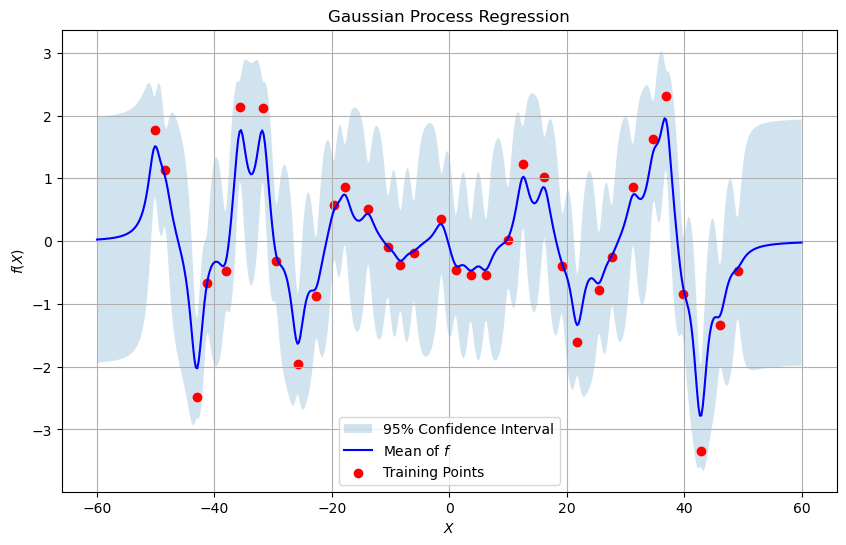
\includegraphics[width=0.7\textwidth]{gp_plot_task1.png}
    \caption{GP with initial kernel parameters.}
\end{figure}

After kernel optimization, the improved GP regression is shown below.

\begin{figure}[H]
    \centering
    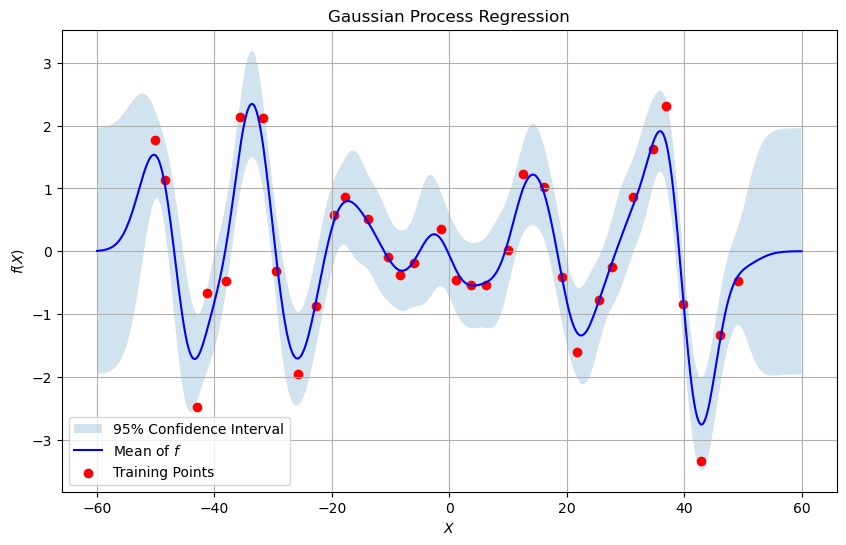
\includegraphics[width=0.7\textwidth]{gp_plot_task2.png}
    \caption{GP with optimized kernel parameters.}
\end{figure}

\subsection{Observations and Discussions}

\subsubsection{Initial Kernel (Task 1)}
The GP model with initial kernel parameters (length\_scale = 1.0, alpha = 1.0) fits the training data well, but the confidence intervals are wide, indicating high uncertainty, especially outside the training range.

\subsubsection{Optimized Kernel (Task 2)}
After optimizing the kernel parameters, the model provides a better fit with narrower and smoother confidence intervals, indicating reduced uncertainty and improved predictive accuracy.

\subsubsection{Discussion}
Kernel parameter optimization improves the GP model’s accuracy and confidence in predictions.

\section{SVM on MNIST}

\subsection{Code}

\subsubsection{Task 1 \& 2}

The imported modules are:

\begin{lstlisting}[language=Python]
import numpy as np
import pandas as pd
import matplotlib.pyplot as plt
from libsvm.svmutil import *
import itertools
\end{lstlisting}

This function loads the training and testing datasets:

\begin{lstlisting}[language=Python]
def load_data():
    # training data
    X_train = pd.read_csv('X_train.csv', header=None).values
    Y_train = pd.read_csv('Y_train.csv', header=None).values.flatten()
    # testing data
    X_test = pd.read_csv('X_test.csv', header=None).values
    Y_test = pd.read_csv('Y_test.csv', header=None).values.flatten()
    return X_train, Y_train, X_test, Y_test
\end{lstlisting}

This function performs a grid search over different combinations of hyperparameters for SVM classifiers.%, testing three kernel types: linear, RBF, and polynomial. The grid search iterates over combinations of hyperparameters and performs cross-validation to determine the best set of parameters. For each kernel type, the following steps are involved:

\[
\text{Accuracy} = \text{svm\_train}(Y_{\text{train}}, X_{\text{train}}, \text{parameters})
\]

Where:

\begin{itemize}
    \item \( \text{Accuracy} \): the cross-validation accuracy of the SVM model for a given set of parameters.
    \item \( Y_{\text{train}} \): the training labels.
    \item \( X_{\text{train}} \): the training features.
    \item \(\text{parameters}\) are determined by the kernel type and the grid of hyperparameters (\(C\), \(\gamma\), and \( \text{degree} \)).
\end{itemize}

\begin{lstlisting}[language=Python]
def grid_search(X_train, Y_train, kernel_type, param_grid):
    # initialize best accuracy and parameters
    best_accuracy = 0
    best_params = None
    param_combinations = list(itertools.product(
        param_grid['C'], 
        param_grid.get('gamma', [0]),
        param_grid.get('degree', [3])
    ))
    
    for C, gamma, degree in param_combinations:
        # set SVM parameters based on kernel type
        if kernel_type == 'LINEAR':
            param = f'-t 0 -c {C} -v 5'
        elif kernel_type == 'RBF':
            param = f'-t 2 -c {C} -g {gamma} -v 5'
        elif kernel_type == 'POLY':
            param = f'-t 1 -c {C} -d {degree} -v 5'
        # train SVM model and get cross-validation accuracy
        accuracy = svm_train(Y_train.tolist(), X_train.tolist(), param)
        # update best accuracy and parameters
        if accuracy > best_accuracy:
            best_accuracy = accuracy
            best_params = (C, gamma, degree)
    
    return best_params, best_accuracy
\end{lstlisting}

% This function defines a custom kernel that combines linear and RBF kernels. The combined kernel is implemented as:

% \[
% K(x, y) = K_{\text{linear}}(x, y) + K_{\text{rbf}}(x, y)
% \]

% Where:

% \begin{itemize}
%     \item \( K_{\text{linear}}(x, y) = \langle x, y \rangle \): the linear kernel, which is simply the dot product of the input vectors \(x\) and \(y\).
%     \item \( K_{\text{rbf}}(x, y) = \exp\left(-\gamma \|x - y\|^2\right) \): the RBF kernel, which measures the similarity between points \(x\) and \(y\) using a Gaussian function with parameter \(\gamma\).
%     \item \(\gamma\) is the RBF kernel parameter controlling the spread of the Gaussian.
% \end{itemize}

% The function is as follows:

% \begin{lstlisting}[language=Python]
% def custom_kernel(kernel1_type, kernel2_type, kernel1_params, kernel2_params):
%     def combined_kernel(x, y):
%         if kernel1_type == 'LINEAR':
%             linear_k = np.dot(x, y)
%         elif kernel1_type == 'RBF':
%             linear_k = np.exp(-kernel1_params['gamma'] * np.sum((x - y)**2))
%         if kernel2_type == 'LINEAR':
%             rbf_k = np.dot(x, y)
%         elif kernel2_type == 'RBF':
%             rbf_k = np.exp(-kernel2_params['gamma'] * np.sum((x - y)**2))
%         return linear_k + rbf_k
%     return combined_kernel
% \end{lstlisting}

This function visualizes the classification results by plotting a bar chart of the accuracy for each kernel type.

% \[
% \text{Accuracy}_{\text{kernel}} = \frac{\text{Correct Predictions}}{\text{Total Predictions}} \times 100
% \]

% Where:

% \begin{itemize}
%     \item \( \text{Accuracy}_{\text{kernel}} \) is the classification accuracy for a given kernel type.
%     \item The accuracy is calculated by comparing the predicted labels with the true labels on the test set.
% \end{itemize}

% The visualization function is:

\begin{lstlisting}[language=Python]
def visualize_results(accuracies, kernel_names):
    plt.figure(figsize=(10, 6))
    plt.bar(kernel_names, accuracies)
    plt.title('SVM Classification Accuracy by Kernel Type')
    plt.xlabel('Kernel Type')
    plt.ylabel('Accuracy (%)')
    plt.ylim(0, 100)
    
    for i, v in enumerate(accuracies):
        plt.text(i, v + 1, f'{v:.2f}%', ha='center')
    
    plt.tight_layout()
    plt.savefig('kernel_comparison.png')
    plt.close()
\end{lstlisting}

The main script performs grid search for each kernel type, trains an SVM with the best parameters, and evaluates on the test set. It then visualizes and prints the final results.

\begin{lstlisting}[language=Python]
# load data
X_train, Y_train, X_test, Y_test = load_data()

# parameter grids for different kernels
param_grids = {
    'LINEAR': {
        'C': [0.1, 1, 10, 100],
    },
    'RBF': {
        'C': [0.1, 1, 10, 100],
        'gamma': [0.001, 0.01, 0.1, 1]
    },
    'POLY': {
        'C': [0.1, 1, 10, 100],
        'degree': [2, 3, 4]
    }
}

# results storage
kernel_results = {}

# Task 1 & 2: Grid Search for Different Kernels
kernel_types = ['LINEAR', 'RBF', 'POLY']
accuracies = []

for kernel in kernel_types:
    # grid search for each kernel
    best_params, best_cv_accuracy = grid_search(
        X_train, Y_train, kernel, param_grids[kernel]
    )
    
    # train with best parameters
    if kernel == 'LINEAR':
        param = f'-t 0 -c {best_params[0]}'
    elif kernel == 'RBF':
        param = f'-t 2 -c {best_params[0]} -g {best_params[1]}'
    elif kernel == 'POLY':
        param = f'-t 1 -c {best_params[0]} -d {best_params[2]}'
    model = svm_train(Y_train.tolist(), X_train.tolist(), param)
    
    # predict and evaluate on test set
    p_label, p_acc, p_val = svm_predict(Y_test.tolist(), X_test.tolist(), model)
    accuracies.append(p_acc[0])
    
    kernel_results[kernel] = {
        'best_params': best_params,
        'test_accuracy': p_acc[0]
    }

visualize_results(accuracies, kernel_types)

# print final results
print("\nFinal Test Set Results:")
for kernel, result in kernel_results.items():
    print(f"{kernel} Kernel:")
    print(f"  Best Parameters: {result['best_params']}")
    print(f"  Test Accuracy: {result['test_accuracy']}%")
\end{lstlisting}

\subsubsection{Task 3}

This is the custom kernel function for Task 3, which combines the linear and RBF kernels. The combined kernel is followed libsvm format, which is shown as below:

\begin{lstlisting}[language=Python]
def compute_custom_kernel(X, Y=None, kernel_type='RBF', gamma=1):
    if Y is None:
        Y = X
    
    if kernel_type == 'LINEAR':
        return np.dot(X, Y.T)
    elif kernel_type == 'RBF':
        X_sq = np.sum(X**2, axis=1)
        Y_sq = np.sum(Y**2, axis=1)
        cross_term = np.dot(X, Y.T)
        return np.exp(-gamma * (X_sq[:, np.newaxis] + Y_sq[np.newaxis, :] - 2 * cross_term))
    
def prepare_kernel_data(labels, kernel, mode='TRAIN'):
    data = []
    
    for i in range(kernel.shape[0]):
        if mode == 'TRAIN':
            instance = {0: i+1}
        else:
            instance = {0: 1}
        
        for j in range(kernel.shape[1]):
            instance[j+1] = kernel[i, j]
        
        data.append((labels[i], instance))
    
    return data

def combined_kernel(X_train, Y_train, X_test, Y_test):
    gamma = 0.1
    
    # Compute combined kernels for training
    linear_train = compute_custom_kernel(X_train, kernel_type='LINEAR')
    rbf_train = compute_custom_kernel(X_train, kernel_type='RBF', gamma=gamma)
    combined_train = 0.5 * linear_train + 0.5 * rbf_train

    # Compute combined kernels for testing
    linear_test = compute_custom_kernel(X_test, X_train, kernel_type='LINEAR')
    rbf_test = compute_custom_kernel(X_test, X_train, kernel_type='RBF', gamma=gamma)
    combined_test = 0.5 * linear_test + 0.5 * rbf_test

    # Prepare the kernel data in libsvm format
    train_data = prepare_kernel_data(Y_train, combined_train, mode='TRAIN')
    test_data = prepare_kernel_data(Y_test, combined_test, mode='TEST')

    # Set up SVM problem and parameters
    prob = svm_problem([item[0] for item in train_data], [item[1] for item in train_data])
    param = svm_parameter('-t 4 -q')
    
    # Train the model
    model = svm_train(prob, param)

    # Predict on test data
    predicted_labels, accuracy, _ = svm_predict([item[0] for item in test_data], [item[1] for item in test_data], model)
    
    print(f'RBF gamma = {gamma}')
    print("Combined Kernel Performance:")
    print(f"Test Accuracy: {accuracy[0]:.2f}%")
    
    return predicted_labels, accuracy

print("\nRunning Combined Kernel (Linear + RBF):")
combined_kernel(X_train, Y_train, X_test, Y_test)
\end{lstlisting}

\subsection{Experiments}

I evaluate the performance of Support Vector Machine classifiers using different kernel types: Linear, Radial Basis Function (RBF), and Polynomial (POLY).

\subsubsection{Hyperparameters}

I Perform a grid search to find the best hyperparameters for each kernel type. The search includes the following hyperparameters:

\begin{align*}
&\text{Linear Kernel: } C = \{0.1, 1, 10, 100\} \\
&\text{RBF Kernel: } C = \{0.1, 1, 10, 100\}, \quad \gamma = \{0.001, 0.01, 0.1, 1\} \\
&\text{Polynomial Kernel: } C = \{0.1, 1, 10, 100\}, \quad \text{degree} = \{2, 3, 4\}
\end{align*}

\subsubsection{Results}

% After performing the grid search for each kernel type, we train the SVM model with the optimal hyperparameters and evaluate its performance on the test set. The following figures present the results for each kernel type.

% The SVM classification performance with the Linear kernel is shown below.

% \begin{figure}[H]
%     \centering
%     \includegraphics[width=0.7\textwidth]{svm_linear_kernel.png}
%     \caption{SVM with Linear Kernel.}
% \end{figure}

% The classification results with the RBF kernel are shown below.

% \begin{figure}[H]
%     \centering
%     \includegraphics[width=0.7\textwidth]{svm_rbf_kernel.png}
%     \caption{SVM with RBF Kernel.}
% \end{figure}

% Finally, the performance with the Polynomial kernel is shown below.

% \begin{figure}[H]
%     \centering
%     \includegraphics[width=0.7\textwidth]{svm_poly_kernel.png}
%     \caption{SVM with Polynomial Kernel.}
% \end{figure}

% \subsubsection{Summary of Performance}

The following table summarizes the best cross-validation accuracy obtained for each kernel type:

\begin{table}[H]
\centering
\begin{tabular}{|c|c|c|}
\hline
\textbf{Kernel Type} & \textbf{Best Accuracy} & \textbf{Best Parameters} \\
\hline
Linear & 95.8\% & (\text{C}=0.1) \\
RBF & 98.16\% & (\(\text{C}=100, \gamma=0.01\)) \\
Polynomial & 97.68\% & (\(\text{C}=100, \text{degree}=2\)) \\
Custom(Linear + RBF) & 95.84\% & (\(\gamma=0.1\)) \\
\hline
\end{tabular}
\caption{Best Accuracy and Parameters for each kernel.}
\label{tab:kernel_performance}
\end{table}

\subsection{Observations and Discussions}

From these results in Table \ref{tab:kernel_performance}, we observe that the RBF kernel achieves the highest classification accuracy.

The Custom kernel combining the Linear and RBF kernels also performs well, which is better than the Linear kernel but slightly lower than the RBF kernel.

\end{document}